\documentclass[11pt,twoside,a4paper]{report}

\usepackage[margin=1in, paperwidth=8.3in, paperheight=11.7in]{geometry}

\usepackage[ruled, vlined, linesnumbered]{algorithm2e}
\usepackage{amsfonts}
\usepackage{amsmath}
\usepackage{changepage}
\usepackage{enumerate}
\usepackage{enumitem}
\usepackage{fancyhdr} % Header
\usepackage{graphicx}

\pagenumbering{arabic}

\begin{document}

\renewcommand{\headrulewidth}{0pt}
\newcommand{\ie}{\textit{i.e.} }
\newcommand{\nats}{\mathbb{N} }
\newcommand{\horizontalline}{\newline\vspace{.3cm}\hfill\makebox[.5\linewidth]{\rule{.5\textwidth}{0.4pt}}\hfill\vspace{.05cm}}

\renewcommand\thetable{\arabic{table}} % figure numbering strategy
\renewcommand\thefigure{\arabic{figure}} % figure numbering strategy

\pagenumbering{roman}

% Header
\pagestyle{fancy}
\fancyhead[L]{Dom Hutchinson (1701111)}
\fancyhead[C]{}
\fancyhead[R]{\today}

% Algorithm environment
\SetArgSty{textnormal}
\DontPrintSemicolon

% Title
\title{Implementing \& Evaluating Space Efficient Algorithms for Detecting Large Neighbourhoods in Graph Streams}
\author{Dom Hutchinson}
\date{\today}
\maketitle
\newpage

\tableofcontents
\newpage

\renewcommand\thechapter{\Roman{chapter}}
\renewcommand\thesection{\thechapter.\roman{section}}
\setcounter{chapter}{1}
\chapter*{Summary/Abstract}
\addcontentsline{toc}{chapter}{Summary/Abstract}

\section{Background}

%\begin{itemize}
%	\item High Degree Detection.
%	\item Large Neighbourhood Detection.
%\end{itemize}

%TODO testing space usage is important as it suggests what will happen when larger graphs are used (the longer we can keep space requirements below RAM space the better).

 % TODO is it ok to define streams & such later
Graphs are a popular way of representing relationships between objects. They are particularly popular within the field of data science \& with the recent movement of \textit{Big Data} it is becoming common to want to deal with large graphs. Moreover, it is common to want to use graphs which cannot be loaded fully onto a computer's RAM and instead require the use of virtual memory. Having to use virtual memory drastically increases request time for data \& thus negatively affects the runtime of algorithms which manipulate these large graphs. Often, in practice, the fastest algorithms for analysing graphs are those which are more space efficient. %rather than those that, in theory, have lower run-time complexity
\par Graph streams have been introduced to reduce the space required to store a graph since they require $O(|E|)$ space, rather than $O(|V|^2)$ space which a traditional matrix representation requires. % TODO define |E| & |V| as edge and vertex sets
Since the number of edges in a graph is cannot be greater than, and is usually much lower than, the square of the number of vertices this is a big improvement. However many graphs still exist which would overflow RAM when loaded in full when in stream form. This is solved by reading the stream one entry at a time as this requires $O(1)$ space. Thus the most space-efficient algorithms for analysing graphs are streaming-algorithms which read instructions sequentially.
\par Graph streams can be used to show the evolution of a graph by insertion \& deleting edges over some time period, in these implementations it is possible for a graph stream to require more space than a matrix representation but since only one instruction is every loaded into the RAM at one time this does not affect the total memory used by a streaming-algorithm. %TODO this might seem out of place (too much detail too early) but I want to make the point that O(|E|) can be greater than O(|V^2|) and this doesn't matter
% TODO perhaps mention that graph streams can show the evolution of a graph (in this case they may have more entries than |V|^2 but doesn't matter since only one entry is every read at a time).
% TODO why single pass??
\horizontalline
\par High degree detection is a common and trivial problem in graph theory. The \texttt{High Degree Detection Problem} entails finding a vertex in a graph with sufficiently high degree. This can be trivially solved for graph streams by keeping counters for the number of edges connected to each vertex and updating the counters after each instruction from the graph stream. % This requires $O(|V|)$ space
\par Although it is useful to identify influential vertices in a graph, it is hard to fully utilise this knowledge without additional information about the neighbourhood of these vertices. Knowing the neighbourhood of a vertex, or at least a subset of it, allows you to make inferences about that node. This leads to the \texttt{Neighbourhood Detection Problem} which is formally stated as

\vspace{.3cm}\begin{adjustwidth}{.3cm}{}\fbox{\parbox{\textwidth}{
\textbf{Problem 1} \texttt{Neighbourhood Detection}.\\
Let $G=(A\cup B,E)$ be a bi-partite graph with vertex sets $A,B$, where $|A|=n$ and $|B|=\text{poly }n$, and edge-set $E$.\\
In $\texttt{Neighbourhood Detection}(G,d,c)$ we are tasked with outputting a vertex from $A$ with at least $d/c$ of its neighbours in $B$. We can assume that $G$ contains at least one node of degree $d$.\\
Here $d\in\nats$ is a threshold parameter \& $c\in(0,1]$ is an approximation parameter.
}}\end{adjustwidth}\vspace{.3cm}

The \texttt{Neighbourhood Detection Problem} is defined for bi-partite graphs in order to generalise the problem. Note that, if we were to define the vertex sets $A,B$ to be equivalent then then the problem holds for every type of graph.
\par Again, the \texttt{Neighbourhood Detection Problem} can be solved trivially by storing the neighbourhoods of every vertex in the graph \& updating them after each instruction from the graph stream. This requires $O(|E|)$ space and can very quickly lead to overflowing the RAM which is undesirable since it means slower run-times for large graphs.

\section{Motivating Applications} %TODO I don't really like this (partly because it is in list form), moreover it isn't really connected in
% NOTE maybe it is best that it is fairly separate from the rest so that it can be skipped over.
%\begin{itemize}
%	\item Real world occurrences \& uses.
%\end{itemize}

There are several real-world applications of the \texttt{Neighbourhood Detection Problem} which motivate investigating it. These are situations where simply knowing highly connected elements of a network is not sufficient.
\begin{itemize}
	\item[-] Given a list of connections within a social network, solving the problem would allow you to not only find \textit{`social influencers'} but those they are connect to too. This allows you to verify that they are indeed a \textit{`social influencers'}, and not someone connected to a lot of bot accounts, and to assess what demographics they have influence over.\\
	For a marketing agency this would mean they don't waste money on people who don't actually have any influence to sell a product, nor on people who have the wrong demographics for a certain product.
	\item[-] Given a list of passengers on public transport you could find people who have come into contact with a lot of people. This is particular relevant in the wake of the COVID-19 outbreak as it could be used to identify people who are likely to have come into contact with infected people. %TODO not a fan of these, might just need fleshing out
	\item[-] Given a list of receipts in a shop you could find the items which are popular, along with which items they are commonly bought with. This information could be used to inform how shelves are stacked and which promotions are run by the store, in order to encourage sales.
	\item[-] Given a log of traffic within a network you could identify which resources are being accessed most often, and by whom. This can be used to inform which resources should be upgraded \& which connections should be prioritised.
\end{itemize}

\section{Structure} %TODO after most the write up
In this paper I am going to implement the two algorithms proposed by Dr Christian Konrad in \cite{orig} for solving the \texttt{Neighbourhood Detection Problem} for graphs streams in a space-efficient manner. I will use this implementation to assess how practical these algorithms are and now to maximise their practicalities.
\par I shall structure this investigation as follows

\begin{itemize}
	\item Insertion-Only Streams
	\begin{itemize}
		\item Layout theory
		\item Discuss features that need to be/can be adjusted in the implementation.
		\item Implement - mentioning any other problems.
		\item Evaluate \& test different combinations of parameters to optimise the practical uses of the algorithm.
		\item Discuss limitations of the implementation. (ie What graphs work)
	\end{itemize}
	\item Repeat for Insertion Deletion.
\end{itemize}

\section{Objectives}
The objectives of this project are
\begin{itemize}
	\item Implement Christian's algorithms and discuss any considerations that need to be taken in doing so.
	\item Tune parameters to make algorithms as practical as possible.
	\item How practical are the algorithms.
\end{itemize}


\renewcommand\thechapter{\arabic{chapter}}
\renewcommand\thesection{\thechapter.\arabic{section}}
\setcounter{chapter}{0}
\chapter{Preliminaries}

\setcounter{page}{1} % restart page counter
\pagenumbering{arabic}

\section{Definitions}

%\begin{itemize}
%	\item Graph
% \item Unweighted, undirected
%	\item Bipartite Graph (Why this wasn't really applied in practice, A=B)
%	\item Graph Stream (Insertion-Only, Insertion-Deletion)
%	\item Neighbourhood, degree & sparsity of a vertex
%	\item Streaming Algorithm
%	\item $1-\varepsilon$ Approximation Algorithm
%	\item TODO Space efficiency??
%\end{itemize}

A \textit{Graph} is a data structure used to represent pairwise relationships between objects. A Graph is defined to have a vertex set, which holds its objects, and an edge-set, which holds the relationship between these objects. Graphs are traditionally visualised with circles for each vertex and lines between vertices that share an edge. There are variations on graphs where the edges are weighted and/or directional. In this project we are only required to deal with undirected, unweighted graphs.
\par A \textit{Bipartite Graph} is a graph whose vertex set can be partitioned into two distinct sets in such a way that all edges in its edge-set run between these partitions \& not within them. % Formally, a graph $G=(V,E)$ where $\exists\ A,B\subset V$ st $V=A\cup B,\ A\cap B=\emptyset$ and $\forall\ (u,v)\in E,\ u\in A\ \&\ v\in B$.
\par The \textit{Neighbourhood} of a vertex in a graph is the set of vertices which it shares an edge with. The \textit{Degree} of a vertex is the size of its neighbourhood. A vertex is $s$ \textit{Sparse} if its degree is less than, or equal to, $s$.
\par A \textit{Graph Stream} is a technique for storing graphs. A graph stream is made up of a series of instructions which are read sequentially and describe how to construct the graph. These instructions describe modifications to the edges of the graph. In this project we are only concerned with two types of graph stream.
\begin{itemize}
	\item \textit{Insertion-Only Streams} where each instruction adds a new edge to the graph.
	\item \textit{Insertion-Deletion Streams} where each instruction either adds a new edge to the graph or removes an existing edge from the graph.
\end{itemize}
Neither of these allow for duplicates of the same edge in the graph, at the same time. Insertion-Deletion streams are used for graphs whose edge-set is dynamic over time, consider a social network where users are able to follow \& un-follow each other. There are other versions of graph streams which all for changes to the weights of edges but these are out of scope for this project. It is noteworthy that insertion-only streams equivalent to insertion-deletion streams which have no deletions. This means that they can be implemented in exactly the same way. % TODO maybe state that these are equivalent to the above if we treat 0 weight to be no edge & anything else to be an edge %TODO maybe mention when order is important (or can represent time)
\par \textit{Streaming Algorithms} are algorithms which are designed to take a stream of sequential instructions as their input. Streaming algorithms can be very space-efficient since only one instruction is read at a time, requiring constant space. Typically streaming algorithms aim to only require a single pass of the input stream so that you can extend the input stream without having to restart the algorithm. Single-pass streaming algorithms are online algorithms. %TODO make the mention of online algorithms more succinct
\par An \textit{$\alpha$-Approximation Algorithm} is an algorithm which returns a result within an $\alpha$ factor to the optimal solution to the problem. Algorithms which solve the \texttt{Neighbourhood Detection Problem} are $\frac1c$-approximation algorithms since they only return $d/c$ of the neighbours of a vertex which we know to have at least $d$ neighbours.

\section{Technologies}
%\begin{itemize}
%	\item C++
%	\begin{itemize}
%		\item Low level
%		\item Memory manipulation
%		\item Faster
%		\item Perhaps something about why not java or python etc.
%	\end{itemize}
%	\item Standard library online
%\end{itemize}
For the implementations in this project I chose to use C++. I initially considered using either python or C++, as they work in the object-orientated paradigm and I am proficient in them. I chose to go with C++ (specifically \texttt{C++11}) as it allows for more control with memory management and typically faster run-times. For this project the memory management is more important as I am looking to evaluate the space-efficiency of algorithms and being able to control their memory allocation means I can identify each time a change occurs to the amount of memory being used. The faster run-times is important when evaluating the practicalities of using these algorithms, as longer run-times make algorithms less practical.
\par I limited myself to using the \textit{C++ Standard Library} (\texttt{std}) as the underlying implementations of this library are well document. This was particularly important for the abstract data types I used as I could check what the underlying implementations and adjust my evaluation accordingly. When implementing randomness I used the \texttt{<random>} module of \texttt{std} and seeded the generators with the current time so that each run would have a different generator.

\section{Evaluation Techniques}

% TODO expectations
%\begin{itemize}
%	\item What features are tested (time \& space)? How?
%	\item Against naïve algorithm.
%	\item Insertion-Only v Insertion-Deletion algorithm for insertion-only streams.
%\end{itemize}

%TODO should this be in the future tense (eg in this paper i will)
%TODO maybe keep this more vague and move the details to their respective sections
%TODO talk about verifying my results
%TODO typical test = vary c between [3,20]. set d=max degree

When evaluating these algorithms there were three main parameters which needed to be tested for: success-rate; time-taken; and, space-used. These are all interconnected and come with their own trade-offs. Typically, the changes to space-used \& time-taken when different strategies are implemented occur in the same direction but at different rates. Whereas, you expect success-rate to go in the opposite direction as the algorithm is using fewer resources.
For these particular algorithms the success rate always remained high but for some setups it takes a lot longer to find a solution. %TODO do I means this??
\par The evaluation process of each algorithm can be broken into two stages. First, I evaluated possible efficiencies to the underlying implementation. The changes tested at this stage did not affect the success-rate of the algorithms but did, in some cases, have a drastic effect on the amount of resources used by each algorithm. Second, I evaluated different set-ups for the parameters of the algorithm. This stage involved a lot more \textit{tuning} of values \& strategies as these affected the logic of the algorithm resulting in trade-offs between resource requirements \& success-rate. The changes in the first were a lot more general \& there was little variation in the results seen for different graph types, whereas in the later stage I had to consider different graph types.
\par I used a global variable to count the space used by different components of the algorithms (as well as the algorithm as a whole) and a timer to evaluate the run-time. For each variation I ran the tests multiple times, recording the results of each run. Typically for testing I set $d$ to be the maximum degree of the graph as these algorithms are typically used to investigate the nodes of greatest degrees in a graph, and I would then vary the approximation factor $c$ as seem reasonable for the given graph.


\subsection{Generating Graphs}

%\begin{itemize}
%	\item How graphs streams are represented.
%	\item Different graph types.
%	\item Generating graphs
%	\item Hard to have wide variety of node degrees.
%	\item Acquired from SNAP.
% \item Graph pre-processing (.vertices file).
%	\item Programs to verify success (ie returned neighbourhood is valid).
%\end{itemize}
For this project I required a number of graphs to evaluate my programs with. By the nature of the algorithms these graphs had to be undirected \& unweighted bi-partite graphs. The bi-partite requirement is unimportant as any graph can be treated as bi-partite by making the vertex set partitions copies of each other.
\par I implemented programs to generate graphs with specific properties which I wanted to test, namely graphs with high disparity in the degree of each node (such as star graphs) and graphs with no disparity between degrees (such as complete graphs). % TODO more justification
I implemented the following programs.
\begin{itemize}
	\item \texttt{completeGraph.cpp} - Generates a graph stream for a complete graph.
	\item \texttt{randomGraph.cpp} - Uses a Bernoulli distribution to determine whether two vertices share an edge in an insertion-only stream, and a poisson distribution to determine how many insertions \& deletions occur between each pair of vertices.
	\item \texttt{starGraph.cpp} - Generates a graph stream for a star graph.
\end{itemize}
All these programs take parameters for the number of vertices and \texttt{randomGraph.cpp} takes parameters for the proportion of edges. Additionally these, programs are able to generate insertion-only or insertion-deletion streams but the final graphs defined by the streams generated by \texttt{completeGraph.cpp} \& \texttt{starGraph.cpp} are always of the appropriate shape. %TODO reword this
%TODO I found it hard to have a wide variety of node degrees
\par I wanted some graphs generated from the real-world so that I could test the algorithms on the sort of data sets they are most likely to be used on. I found a collection of large graph streams, from different applications, in the \texttt{Stanford Network Analysis Project} (\texttt{SNAP}) datasets collection \cite{SNAP}. %TODO I chose social network ones??
The vertices in the instructions of these graph streams were not ordered meaning that these graphs are not strictly bi-partite. % TODO better explanation?
This meant I needed to change my implementations slightly such that both ends of the edge are treated as $A$-vertices. This is equivalent to having a bi-partite graph where the $A$ \& $B$ vertex sets are copies of each other, which is perfectly fine.
\par The graphs from \texttt{SNAP} were all insertion-only streams so I wrote a program which would generate an insertion-deletion stream from them by adding a defined proportion of deletion instructions throughout the stream. This program maintained the property that no edge was deleted before it was inserted.
\par I wrote \texttt{utility.cpp} to perform a number of tasks to these graphs. Most notably, it can produce a file which lists the final degree of every vertex in the graph stream and it can verify whether a given set is a subset of the neighbourhood of a given vertex. I used the later function to verify the outputs generated by implementation of Dr Konrad's algorithms.
%TODO table of used graphs

%TODO confirm values for gplus_large
\begin{center}
	\begin{table}[h]
		\caption{Details of graphs used during evaluation}
		\tiny
		\begin{tabular}{|l|l|l|l|l|l|l|l|}
			\hline
			\textbf{Name}&\textbf{Source}&\textbf{Type}&\textbf{\# Vertices}&\textbf{\# Edges}&\textbf{\# Instructions}&\textbf{Max Degree}&\textbf{File Size}\\
			\hline
			$\mathtt{facebook\_small}$&SNAP&Insertion-Only&52&292&-&36&3 KB\\
			$\mathtt{facebook\_small\_deletion}$&Generated&Insertion-Deletion&52&258&326&33&5 KB\\
			$\mathtt{facebook}$&SNAP&Insertion-Only&747&60,050&-&586&587 KB\\
			$\mathtt{facebook\_deletion}$&Generaetd&Insertion-Deletion&747&53,457&66,643&522&846 KB\\
			$\mathtt{gplus}$&SNAP&Insertion-Only&12,417&1,179,613&-&5,948&53 MB\\
			$\mathtt{gplus\_deletion}$&Generated&Insertion-Deletion&12,417&1,049,309&1,309,917&4,998&60 MB\\
			$\mathtt{gplus\_large}$&SNAP&Insertion-Only&102,100&30,238,035&-&104,947&1.3 GB\\
			$\mathtt{1000vertices}$&Generated&Insertion-Only&1,000&246,676&-&984&2 MB\\
			$\mathtt{doublepoisson05ID}$&Generated&Insertion-Deletion&10,000&8,639,534&24,452,736&4,977&305 MB\\
			$\mathtt{1000star}$&Generated&Insertion-Only&1,000&999&-&999&9 KB\\
			$\mathtt{1000starID}$&Generated&Insertion-Deletion&1,000&999&1,023&999&11 KB\\
			$\mathtt{1000complete}$&Generated&Insertion-Only&1,000&499,500&-&999&4 MB\\
			$\mathtt{1000completeID}$&Generated&Insertion-Deletion&1,000&499,500&509,524&999&5 MB\\
			\hline
		\end{tabular}
	\end{table}
\end{center}

\chapter{Insertion-Only Streams}

\section{Degree-Based Reservoir Sampling}

\texttt{Degree-Based Reservoir Sampling} is a technique for uniformly sampling a subset from the set of vertices whose degrees are greater than a specified minimum bound, while storing part of the neighbourhood for each of the sampled nodes. This sample is known as the \textit{reservoir}.

\par \texttt{Degree-Based Reservoir Sampling} takes three parameters: the lower bound for the degree of vertices at which to start sampling, $d_1\in\nats$; the maximum neighbourhood size to store for each vertex, $d_2\in\nats$; and the maximum reservoir size, $s\in\nats$. \texttt{Degree-Based Reservoir Sampling} succeeds if it finds a neighbourhood of size $d_2$.

%\par Degree-based reservoir sampling \underline{only} works for insertion-only graph streams.

\par Three data stores are used in \texttt{Degree-Based Reservoir Sampling}: a map of the degree of every node in the graph; a set for the reservoir; and a set for edges incident to the vertices in the reservoir.

\par The reservoir has an invariant that at any point in time it contains a uniform sample of the vertices whose degrees are known to be greater than $d_1$ at that time. This invariant is maintained by controlling how vertices are added to the reservoir. The first time the degree counter for a vertex $v$ surpasses $d_1$ we consider whether to add $v$ to the \textit{reservoir}. There are two cases
\begin{itemize}
	\item If the reservoir is \underline{not} full (ie its size is less than $s$) then we add $v$ to the reservoir.
	\item Otherwise, if the reservoir is already full then we use a Bernoulli random variable with probability $p=\frac{x}s$, where $x$ is the size of the reservoir. If this random variable succeeds then we pick, uniformly at random, a vertex $u$ currently in the reservoir and replace it with $v$. We remove all the edges in the edge set which are incident to $u$ and no other vertices in the reservoir.
\end{itemize}
If $v$ is not added to the reservoir at this time, it never will be in the future. Note that in the case that the reservoir is full \& $v$ is inserted into it, $v$ is replacing an element that was in the reservoir and any progress which has been made towards finding a neighbourhood for that vertex is annulled in doing so. The amount of progress is not taken into account \& thus if there is a high turn-over of elements in a reservoir then less progress is made towards finding a neighbourhood for each of them. This is something I will look into during the evaluation.

\par Whenever an edge is encounter which is in incident to a vertex in the reservoir then we add it to the set of edges. The sampler runs until the graph stream is exhausted at which point it returns, uniformly at random, one of the neighbourhoods of sufficient size.

\par \texttt{Degree-Based Reservoir Sampling} only works on insertion-only streams as it does not account for when the degree of a vertex falls below the threshold, after being sampled. This means the reservoir is not necessarily a uniform random sample of the vertices with degree $\geq d_1$. %TODO is this sufficient

\par For this project we are interested in how \texttt{Degree-Based Reservoir Sampling} can be implemented for bi-partite graphs, specifically we want to sample from the $A$-vertices of the graph. For a bi-partite graph with $n$ $A$-vertices \texttt{Degree-Based Reservoir Sampling} requires $O(n\log n+sd_2\log n)$ space, assuming $O(\log n)$ space is required to store an edge or a vertex, since it stores a degree counter for every $A$-vertex and at most $d_2$ edges for each of the $s$ vertices in the reservoir. \textbf{Algorithm 1} outlines pseudocode for \texttt{Degree-Based Reservoir Sampling} on a bi-partite graph.

\begin{algorithm}
	\caption{\texttt{Degree-Based Resevoir Sampling}$(d_1,d_2,s)$}
	\SetKwInOut{Require}{require}
	\Require{Lower degree bound $d_1\in\nats$, Upper neighbourhood bound $d_2\in\nats$, Reservoir size $s\in\nats$, Insertion-only stream $\{(a_0,b_0),\dots,(a_n,b_n)\}$}
	$D\leftarrow\{\}$ \tcp*{Degree counter}
	$R\leftarrow\{\}$ \tcp*{Reservoir}
	$S\leftarrow\{\}$ \tcp*{Collected edges}
	$x\leftarrow0$\tcp*{\# nodes of degree$\geq d_1$}
	\For{$i\in[0,n]$} {
		$D[a_i]\leftarrow D[a_i]+1$\tcp*{Increment degree counter}
		\If{$D[a_i]\equiv d_1$}{
			\tcp{Consider inserting $a_i$ to reservoir}
			$x\leftarrow x+1$\\
			\If{$|R|<s$} {
			\tcp{Reservoir is not full}
			$R\leftarrow R\cup\{a_i\}$
			} \Else {
				\tcp{Reservoir is full}
				\If{\texttt{Bernoulli}$\left(\frac{s}x\right)$} {
					Let $a'$ be a uniform random element of $R$\tcp*{Element to replace}
					Delete edges in $S$ incident to $a'$\\
					$R\leftarrow(R\backslash\{a'\})\cup\{a\}$\tcp*{Swap $a_i$ and $a'$}
				}
			}
		}
		\If{$a_i\in R$}{
			$S\leftarrow S\cup(a_i,b_i)$\tcp*{Store edge}
			\If{$D[a_i]\equiv d_1+d_2$} {
				\Return{edges in $S$ incident to $a_i$\tcp*{Success}}
			}
		}
	}
	\Return{FAIL\tcp*{No sufficient neighbourhoods found}}
\end{algorithm}

\section{Proposed Algorithm}

%\begin{itemize}
%	\item Assumptions: no duplicate edges (can mitigate cases when this would be required by being smart)
%	\item Insertion stream neighbourhoods cannot be diminished over time.
%	\item Possibility of failure (missed edges) \& mitigation
%	\begin{itemize}
%		\item Theorem 3.2 (probs not proof)
%	\end{itemize}
%	\item Theoretical space requirements
%\end{itemize}

The \texttt{Neighbourhood-Detection Problem} can be solved using \texttt{degree-based reservoir sampling} sampling by setting $d_2=\frac{d}c$. The question remains as to what to set $d_1$ and $s$ to in order to get a high probability of success. In \cite{orig} it is proven that setting $s=\lceil\ln(n)\cdot n^{\frac1c}\rceil$ and using $c$ \texttt{degree-based reservoir samplers} each with a different lower bound, incremented from $\frac{d}c$ to $d$ stepping by $\frac{d}c$ each time, results in a high probability of success. The algorithm suggested by Dr. Konrad runs the samplers in this way, with $s$ set to $\lceil\ln(n)\cdot n^{\frac1c}\rceil$. The proposed algorithm returns, uniformly at random, any of the neighbourhoods return by a successful sampling. %TODO proof? Say it's insertion-only
\par Each of the $c$ samplers requires $O(n\log n+sd_2\log n)$ space. Since the degree map can be shared between samplers the total space is $O(n\log n+c\cdot sd_2\log n)=O(n\log n+c\lceil\log(n)n^{\frac1c}\rceil\frac{d}c\log n)=O(n\log n+n^{\frac1c}d\log^2n)$. %TODO with algorithm parameter values
The proposed algorithm does require you to know the number of vertices in the graph stream before running the algorithm, or at least the log of it. If this is unknown then it is quick to run through the whole stream \& build a set of vertices in the graph. This requires $O(n\log n)$ space, assuming $O(\log n)$ space is required to store a vertex. In many real-world scenarios this number (or a good approximation) will be known due to it being important for other tasks.
\par \textbf{Algorithm 2} is the algorithm proposed in \cite{orig} for solving the \texttt{Neighbourhood-Detection Problem} for insertion-only streams.\\

\begin{algorithm}
	\caption{One-pass $c$-Approximation Insertion-Only Streaming Algorithm for $\mathtt{Neighbourhood\ Detection}$}
	\SetKwInOut{Require}{require}
	\Require{Space $s$, degree bound $d$.}
	$s\leftarrow\lceil\log(n)\cdot n^{\frac1c}\rceil$\\
	\For{$i\in[0,c-1]$\text{\textbf{ in parallel}}} {
		$(a_i,S_i)\leftarrow\mathtt{Deg}\mbox{-}\mathtt{Res}\mbox{-}\mathtt{Sampling}\left(\max\left\{1,i\cdot\frac{d}{c}\right\},\frac{d}c,s\right)$
	}
	\Return{\small Uniform random neighbourhood $(a_i,S_i)$ \text{from successful runs}}
\end{algorithm}

\section{Implementation}

I centred my implementation around working for the graph streams from \textit{SNAP} \cite{SNAP} as they came from real-world sources \& thus are very important for testing the real-world practicalities of the proposed algorithm. These graph streams are not formatted in a strictly bi-partite way. I adjusted \texttt{degree-based reservoir sampling} to account for this by by repeating \texttt{lines 6-19} of \textbf{Algorithm 1} after the end of the \texttt{for} loop, with all occurrences of $a_i$ replaced by $b_i$.
%TODO something about implementing in parallel. Nah
\vspace{.3cm}\newline
After an initial implementation I considered two alterations which could be made:
\begin{enumerate}
	\item \textit{Early Termination} - Returning the first neighbourhood of sufficient size, rather than uniformly sample from all which succeed; and,
	\item \textit{Shared Edge-Set} - Having all samplers share an edge-set, rather than each have one each.
\end{enumerate}

\noindent\textbf{Algorithm 2} states to run through the whole stream before sampling uniformly from the successfully returned neighbourhoods, but this is not necessary to fulfil \texttt{neighbourhood detection}. Returning the first neighbourhood of size $\frac{d}c$ is sufficient for solving the problem. Implementing this should reduce run-time as only part of the stream is being used and should reduce space used by the edge-sets in reservoir sampling as no data is stored after the first solution is found. As this change terminates at the first success there is no change to the success rate of the algorithm. One down side is that you will likely get less variety in the returned neighbourhoods as the algorithm will not encounter every vertex which meets the degree requirements, however this is not relevant to the problem.

\par I implemented this change and evaluated the implementation at different values of $c$. Space-requirements more than halved in every instance. For graphs with the least variation in degree distribution space-requirements decreased by more than $97\%$ after early termination was introduced (as there are many vertices with valid neighbourhoods). Introducing early termination meant that run-times reduced as $c$ increased, whereas before run-times increased with $c$. These results are shown in \texttt{Figure 1} \& \texttt{Figure 2}. These are really good results, so I implemented this change going forward. %TODO explain reasons behind these results
%TODO comment about effect on space used by reservoirs vs degree map
%TODO this change means that time taken is now a measure of success as failure is (basically) the only time the whole stream is run through

\vspace{.3cm}\begin{adjustwidth}{.3cm}{}\fbox{\parbox{\textwidth}{

\textbf{Lemma 2.1} If \textbf{Algorithm 2} terminates after the first sufficient neighbourhood it finds, no vertex occurs in multiple reservoirs at the same time.\\

% TODO a proof by contradiction
\textit{Proof (by contradiction)} Let $v$ be a vertex in the graph stream. Suppose, without loss of generality, that $v$ is a member of the reservoirs of both \texttt{Deg-Res-Sampling}$(\frac{d}{c},\frac{d}{c},s)$ \& \texttt{Deg-Res-Sampling}$(\frac{2d}{c},\frac{d}{c},s)$. This means that $v$ was sampled twice, after encountering the $\frac{d}c^\text{th}$ \underline{and} $\frac{2d}c^\text{th}$ edge incident to $v$ in the stream. After sampling $v$ for the first time, encountered edges which are incident to $v$ are stored. This means that by the time $v$ is sampled for the second time $\frac{2d}c-\frac{d}c=\frac{d}c$ edges incident to $v$ have been stored. This is a sufficient neighbourhood for \textbf{Algorithm 2} to terminate. This is a contradiction since termination occurs before the second sampling occurs.$\hfill\square$

}}\end{adjustwidth}\vspace{.3cm} %TODO refine

\par A consequence of \textbf{Lemma 2.1} is that an edge is only stored in multiple edge sets if its endpoints are sampled by different samplers. %TODO mention this is rare
This means that introducing a shared edge-set for all samplers will not have a great effect on the space requirements of \texttt{Algorithm 2}.
\par However, the alterations to the implementation which would have to made to allow for a shared edge-set could introduce time savings. Namely, I would need a data-structure which tells me \underline{precisely} which reservoir each vertex is in that so I know the appropriate value of $d_1$ in \texttt{Algorithm 1:Line 18}, otherwise improper termination could occur. An appropriate data-structure for this would be a \texttt{map} from each vertex to a bitstring whose indices indicate whether the vertex lies in an associated reservoir. With this implementation, inserting or deleting a vertex to/from a reservoir and querying whether a vertex is in a given reservoir becomes querying a map \& then a known bit in a bitstring which both take $O(1)$ time. This \texttt{map} replaces the \texttt{ordered set}s currently used to store the reservoirs of each sampler and thus reduce these action times from $O(\log n)$ to $O(1)$ time. As these actions occur a lot this change should result in a reasonable reduction in run-time. % TODO something about space used to store a vertex in the map vs in sets

\par I implemented this map, along with a shared edge-set, %NOTE even though this shouldn't change much
and ran tests for values of $c\in[3,100]$. These tests showed an ~8\% reduction in run-time when the map \& shared edge-set where introduced. It should be noted that in a few cases the algorithm was slower but <1\% which I think is a reasonable trade off. % TODO maybe include the variance
There were no gains in the space requirements when a shared edge-set was used, nor were there losses. The results can be seen in \texttt{Figure 3} \& \texttt{Figure 4}.
\par Implementing a shared-edge set does not change the logic of the algorithm so does not affect its success rate. Due to the reduction in mean run-time \& no noteworthy changes in space requirements, I recommend implementing this change. %TODO do I mean ``logic''??

%TODO discuss performance against theory
\section{Parameter Tuning}

%\begin{itemize}
%	\item Vary size of reservoir ($s$) \& number of samplers together to find an optimum
%	\item Full optimised against v Naïve.
%\end{itemize}

\par The changes discussed above have been to the implementation of \texttt{degree-bound reservoir samplers}, rather than to the proposed algorithm. This means these changes have had no affect on the success rate of the algorithm. I will now discuss potential changes to the proposed algorithm. These changes will have an effect on the success rate of the algorithm. It is possible that no change in the success-rate will be seen \& rather the change will occur in execution time as more instructions have to be read before a solution is found. I am investigating the practicalities of the algorithm so keeping the run-times usable is a high priority. In \texttt{Algorithm 2} there are two parameters which can be played around with: the number of samplers; and, the size of the reservoirs, $s$.

\par The total sample size, $\left\lceil\ln(n)n^{\frac1c}\right\rceil\times\text{\#\ Samplers}$, is the main factor effecting the space-used by the algorithm as this is the number of vertices it needs to store edges for. Noting that \texttt{Algorithm 2} sets the number of samplers to be $c$ and that $cp\left\lceil\ln(n)n^{\frac1c}\right\rceil\leq c\left\lceil p\ln(n)n^{\frac1c}\right\rceil\ \forall\ p\in[0,1]$ it is apparent that reducing the number of samplers has a greater effect on total sample size, and thus space-used, than reducing sample size by the same proportion. For this reason I investigated the number of samplers first.

\horizontalline

\par When changing the number of samplers we need to consider their lower bounds, $d_1$, too. If the range of vertex degrees which individual samplers sample, $[d_1,d_1+d_2]$, at overlap then duplicate sampling of vertices can occur which offers no advantages \& leads to a reservoir space being wasted. And, if there are gaps between these ranges then there are vertices which may not be sampled. %TODO flesh this out more.
Thus, the best set up is to have the sampling ranges be sequential with no gaps and so when varying the number of samplers we should only add or remove from the endpoints of these ranges. The samplers with lower lower-bounds, $d_1$, start sampling earlier \& from a larger pool. I expect these early samplers to be more important wrt performance gains, than later samplers. It is not necessarily true that the first sampler is the most important as it is sampling from the largest pool and so has the greatest turn-over rate in its reservoir.

\par I ran the following tests to investigate what had a greater effect on performance, removing later samplers or earlier samplers.
\begin{enumerate}
	\item Removing the \underline{first} $x$ samplers from \texttt{Algorithm 2} for $x\in[1,c)$, for $c\in[1,20]$.\\
	\textit{i.e.} Change the \texttt{for} loop in \texttt{Algorithm 2:Line 2} to run for $i\in[x,c-1]$.
	\item Removing the \underline{last} $x$ samplers from \texttt{Algorithm 2} for $x\in[1,c)$, for $c\in[1,20]$.\\
	\textit{i.e.} Change the \texttt{for} loop in \texttt{Algorithm 2:Line 2} to run for $i\in[0,c-x]$.
\end{enumerate}

\par These tests confirmed the hypothesis that the lower a sampler's lower-bound is, the greater the effect of its inclusion on performance. Time-taken increased as more early samplers were removed, and decreased as more late samplers were removed. Comparing the relative difference of these results shows that removing early samplers is more detrimental to performance than including later samplers. This is due to late samplers only starting to sample later \& they may not have begun sampling by the time one of the previous samplers has succeed, terminating the algorithm. When the same proportion of samplers were removed for different values of the approximation factor, $c$, the relative performance was worse for greater values of $c$. This is to be expected as the real number of samplers removed increases with $c$. As expected the space-used decreased whenever more samplers were removed. During the second test some failures did occur when only the first sampler was used on larger graphs.
The results to these tests on \texttt{gplus} can be seen in \texttt{Figure 5} \& \texttt{Figure 6}, results for other graphs followed similar trends.

\par From these tests it is apparent that there are advantages to be found by removing late samplers, but not from removing the earliest. These tests did show that the failure rate does increase when too few of the early samplers are used. Thus I repeated the tests, this time testing when $\leq25\%$ of the earliest samplers were used and ran more repetitions so I could evaluate the failure rate better.

\par This test showed that the success rate was less than 1 only when just the first sampler was used, even on the largest graphs. Even in these cases it was still above $.9$. Since failure only occurs when the whole stream is run through, runs which failed take a lot longer to run than those that succeed (5 minutes compared to $~10$ seconds for \texttt{gplus\_large}). This meant that the implementations which only used the first two samplers were quicker on average.

\par The success rate when only the first sampler was used was lower for larger graphs, but was higher for greater values of the approximation factor. In all my tests, running just the first two samplers provided the best results. However, the largest graph I tested on only contains $~100,000$ vertices so it is likely this may not hold for significantly larger graphs. I suggest using the first $\mathtt{max}\left(2,\left\lceil\frac15\ln n\right\rceil\right)$ samplers. As we don't want the sampling ranges to overlap we need to add a restriction that the number of samplers is never greater than the approximation factor, giving the number of samplers used as $\mathtt{min}\left(c,\mathtt{max}\left(2,\left\lceil\frac15\ln n\right\rceil\right)\right)$.

\par When tested on \texttt{gplus\_large} introducing this change halved run times for tight approximation factors ($c\in[3,10]$), for looser approximation factors time-savings of over 90\% were made. This is because the number of samplers removed increases as the value of the approximation factor increases. This implementation had little effect on space-usage when compared to the implementation before the number of samplers was reduced, whilst maintaining a perfect success rate. The lack of change in space-usage shows that these later samplers were not being used and were just adding wasted computation time. These results can be seen in \texttt{Figure 7} \& \texttt{Figure 8}.
%TODO something about how the fact that space hasn't changed much means later samplers weren't coming into play often & thus sample size is unlikely to be important.
%TODO comment of special cases
\horizontalline
\par Removing later samplers had little effect on the space used by the algorithm. This is due to these samplers not getting the chance to sample very often as the algorithm often terminated before many vertices of sufficient degree were encountered. This means that reducing the size of those samplers would have had virtually no affect on the performance of the algorithm. This helps justify optimising the number of samplers before the sample sizes. The previous optimisation means that very few samplers are being run so it is unlikely that any great improvements will be found, if any, when reducing sample size.

\par Decreasing the sample size $s$ means less edges are stored, reducing space requirements, but increases the turn-over rate of the elements in the reservoir as the probability a vertex is sampled is the same but the sample size is smaller. The greater turn-over rate is detrimental to the success of the algorithm as it more likely for a vertex to be removed when it is close to succeeding. For very low sample sizes it is likely that the success rate of the algorithm will remain high, but the run-times will be dramatically increased.

\par I tested having the sample size set to between $10\%$ and $200\%$ of the proposed size, at $10\%$ increments, in order to get an overview of how sample size affects performance. This test showed a positive linear relationship between sample size \& space-used. The only inference that could be drawn from sample-size \& time-taken is that there is a point at which time-taken dramatically increases, this is the point where the algorithm fails to return a result. Overall, there is no clear strategy to improving the algorithm by varying the sample size. There may have been if we had not already reduced the number of samplers, but for reasons discussed earlier it is justified to optimise the number of samplers first. These results can be seen in \texttt{Figure 9} \& \texttt{Figure 10}.\\

%TODO mention theoretical space efficieny of this (should be same as before)
\par Here is \textbf{Algorithm 2} rewritten to include the proposed parameter optimisations
\begin{algorithm}
	\caption{One-pass $c$-Approximation Insertion-Only Streaming Algorithm for $\mathtt{Neighbourhood\ Detection}$}
	\SetKwInOut{Require}{require}
	\Require{Space $s$, degree bound $d$.}
	$s\leftarrow\lceil\log(n)\cdot n^{\frac1c}\rceil$\\
	$n_s\leftarrow\min\left(c,\max\left(2,\left\lceil\frac15\ln(n)\right\rceil\right)\right)$\\
	\For{$i\in[0,n_s]$\text{\textbf{ in parallel}}} {
		$(a_i,S_i)\leftarrow\mathtt{Deg}\mbox{-}\mathtt{Res}\mbox{-}\mathtt{Sampling}\left(\max\left\{1,i\cdot\frac{d}{c}\right\},\frac{d}c,s\right)$
	}
	\Return{\small Uniform random neighbourhood $(a_i,S_i)$ \text{from successful runs}}
\end{algorithm}

%TODO rewrite algorithm 2 with these parameter optimisations
\section{Evaluation}

%Run the following instances on different graphs \& compare
%\begin{itemize}
%	\item Initial implementation (no tuning, not quit early, not sharing)
%	\item Implementation with early quitting & shared edges
%	\item Implementation with tuned algorithm parameters
%	\item Naïve Implementation
%\end{itemize}
% Compare max space to size of edges file
% Identify which change had what effect (to space, time, success)
%TODO 1000star is useful as there is only one valid solution
To evaluate my final implementation I compared its performance to that of different stages of the optimisation and to a naïve implementation of the algorithm. These different stages were
\begin{enumerate}[label=\roman*)]
	\item Initial Implementation - No early termination, shared edge-set or sampler removal. %insertionStreamsNotQuitEarly
	\item After Technical Optimisation - Implements early termination \& a shared edge-set. %insertionStreamsSharedEdgeSet
	\item After Algorithmic Optimisation - Implements early termination, shared edge-set and sampler removal. %insertionStreamsRemovedSamplers
\end{enumerate}
The naïve algorithm I used is given in \texttt{Algorithmn 4}. This aproach records the neighbourhood of every encountered vertex \& returns the first one which surpasses the $\frac{d}c$ threshold. This algorithm will always succeed as there is a requirement that at least one vertex in the graph is of degree, at least, $d$. As the naïve algorithm terminates at the first neighbourhood of sufficient size \& uses all edges in the stream up to that point, it is guaranteed to find the first vertex with a sufficient neighbourhood. This means the naïve algorithm is very quick, provided its space-usage is within the memory allocated to the algorithm. In the worst case, where the last element is the only element of degree $\frac{d}c$ and all other $n-1$ elements have degree $\frac{d}c-1$, $\frac{d}{c}+(n-1)(\frac{d}c-1)\in O(n\frac{d}c)$ space is required. The average case has the same complexity and the best case, where the first $\frac{d}c$ instructions are incident to the same vertex, has $O(\frac{d}c)$ space-complexity.
\begin{algorithm}
	\caption{Na\"ive Single-Pass Insertion-Only Streaming Algorithm for Neighbourhood Detection}
	\SetKwInOut{Require}{require}
	\Require{Stream $\{(s_0,t_0)\dots(s_n,t_n)\}$, degree bound $d$, precision bound $c$}
	$N\leftarrow\{\{\}\}\ \{\text{neighbourhoods}\}$\\
	\For{$i=0\dots n$} {
		append $t_i$ to $N[s_i]$\tcp*{Insert neighbour}
		\If{\text{size}($N[s_i])\geq d$} {
			\tcp{Sufficiently large neighbourhood found}
			$S\leftarrow \{N[s_i][0],\dots,N[s_i][\frac{d}{c}]\}$\tcp*{First $\frac{d}c$ elements of neighbourhood}
			\Return{($s_i,S$)}
		}
	}
	\Return{FAIL}\tcp*{No neighbourhoods found}
\end{algorithm}

% TODO a table of results??

\par The empirical results showed that the space usage for the naïve algorithm was significantly greater than that of any of the proposed implementations. This high usage of space could be seen in practice as the naïve algorithm did not return a solution when the approximation factor was 2 for \texttt{gplus\_large}, even after 3 hours of computation. For all the graphs, except \texttt{1000star}, the implementations of the proper algorithm used less than the stream file size for all approximation values. For the largest graph tested, \texttt{gplus\_large}, only $13.7\%$ of the stream file size was required to find a 2-approximation using the initial implementation. After my optimisations this was reduced to $1.39\%$. The space-usage results for \texttt{gplus}, the largest file which the naïve algorithm was usable on, are given in \texttt{Figure 11} with the results normalised by the stream's size (51,839 KB).

%TODO comment on performance compared to theory

\par As I supposed the naïve algorithm was generally the fasted algorithm, in the cases where it succeeded, as it always used the fewest number of instructions required. My final implementation, after algorithmic tuning, was between 50-100\% slower than the naïve implementation in these cases. My final implementation is useably quick: when run on \texttt{gplus\_large} it took ~150s to find a solution when $c=2$ and less than a minute for $c\geq5$. The naïve algorithm being quicker is irrelevant for this evaluation as it fails to terminate for larger files due to its space inefficiency. The time taken results for \texttt{gplus}, the largest file tested, are shown in \texttt{Figure 12}.

\section{Conclusion}

\par During the optimisation process I made three changes which helped improve the performance of the algorithm: I made the algorithm return the first neighbourhood it encountered of sufficient degree. This reduced both time \& space requirements as less of the graph stream was consumed; I set up the samplers to share an edge set. This was meant to reduce space requirements, but due to early termination duplication of edges was now very rare. This change did reduce run times as the time complexity for operations on reservoirs was reduced from $O(\log n)$ to $O(1)$; And, I reduced the number of samplers being run by removing most of the late samplers which were very rarely used (due to early termination). This change had little effect on space requirements, but did reduce run-time substantially, especially for high values of the approximation factor. After all these changes the algorithm maintained a perfect success rate during all final tests.

\par I proposed changing the sample size of each reservoir. Preliminary tests presented no strategies which could consistently improve one performance metric without unreasonably affecting another. Thus this idea was not implemented. It is likely that if the number of samplers had not been reduced by as much as then varying the sample size could have had a positive effect on the algorithm, but the gains from reducing the number of samplers are so good they must be incorporated.

\par The final evaluation shows that the proposed algorithm is much more space-efficient that a naïve approach \& even for close approximations of large streams my final implementation uses less than $6\%$ of the file size and for $c\geq5$ it uses $\leq1\%$. This space efficiency increases the maximum file size at which the algorithm is usable, with without requiring virtual memory. The run-times of my final implementation are very usable with solutions being found in a couple of minutes for close approximations ($c\in[2,4]$) and taking significantly less time for loser approximations. Whilst evaluating my final implementation no failures occurred. All these results show that the proposed algorithm for insertion-only streams \underline{is} indeed practical in real-world scenarios.

\chapter{Insertion-Deletion Streams}

\section{$L_0$ Sampling}

\begin{itemize}
	\item L0 sampling uniformly samples from the non zero elements of a vector.
	\item In this setting we consider the edge vector of each vertex (indicates which vertices it shares an edge with).
	\item The formally proposed algorithm.
\end{itemize}

\subsection{Implementation}
%NOTE this was hard
\begin{itemize}
	\item How to L0 sample a graph stream
	\item Hash functions are hard (trade off due to dodgy hash generation).
\end{itemize}

\section{The Algorithm}

\begin{itemize}
	\item There are two algorithms.
	\item Scenarios when each algorithm is most suitable.
	\item L0 samplers in parallel (lots of pre-allocated space).
\end{itemize}

\begin{algorithm}[H]
	\caption{One-pass $c$-approximation Insertion-Deletion Streaming Algorithm for $\mathtt{Neighbourhood\ Detection}$. \text{(Vertex Sampling)}}
	\SetKwInOut{Require}{require}
	\Require{Space $s$, degree bound $d$.}
	Let $x=\max\left\{\frac{n}{c},\sqrt{n}\right\}$\\
	Sample a uniform random subset $A'\subseteq A$ of size $10\ x\ln n$ of vertices.\\
	\For{$a\in A'$} {
		Run $10\frac{d}{c}\ln n$ $l_0$-samplers on the set of edges incident to $a$.
	}
	\Return{\small Any neighbourhood of size $\frac{d}{c}$ among the stored edges, if there is one.}
\end{algorithm}

\begin{algorithm}[H]
	\caption{One-pass $c$-approximation Insertion-Deletion Streaming Algorithm for $\mathtt{Neighbourhood\ Detection}$. \text{(Edge Sampling)}}
	\SetKwInOut{Require}{require}
	\Require{Space $s$, degree bound $d$.}
	Let $x=\max\left\{\frac{n}{c},\sqrt{n}\right\}$.\\
	Run $10\frac{nd}{c}\left(\frac1x+\frac1c\right)\ln (nm)$ $l_0$-samplers on the set of edges incident to $a$.\\
	\Return{\small Any neighbourhood of size $\frac{d}{c}$ among the returned edges, if there is one.}
\end{algorithm}

\section{Implementation}
%TODO will be shorter than for Insertion-only

\begin{itemize}
	\item L0 samplers in parallel
	\begin{itemize}
		\item require lots of preallocated space (know how much space is used at start of algorithm)
	\end{itemize}
	\item Require list of vertices before vertex sampling.
\end{itemize}

\section{Parameter Tuning}

\begin{itemize}
	\item gamma \& delta for L0 sampling
	\item vertex sample size \& samplers per vertex
	\item num edge samplers
\end{itemize}

\section{Evaluation}

% L0 space v sample size space

\begin{algorithm}[H]
\caption{Na\"ive Single-Pass Insertion-Streaming Algorithm for Neighbourhood Detection}
\SetKwInOut{Require}{require}
\Require{Stream $\{(w_0,s_0,t_0)\dots(w_n,s_n,t_n)\}$, degree bound $d$, precision bound $c$}
$N\leftarrow\{\{\}\}\ \{\text{neighbourhoods}\}$\\
\For{$i=0\dots n$} {
	\If{$w_i\equiv1$}{append $t_i$ to $N[s_i]$\tcp*{Insertion instruction}}
	\ElseIf{$w_i\equiv-1$}{remove $t_i$ from $N[s_i]$\tcp*{Deletion Instruction}}
}
\tcp{Look for a sufficiently large neighbourhood}
\For{$s_i\in N.keys$}{
	\If{\text{size}($N[s_i])\geq d$} {
		\tcp{Sufficiently large neighbourhood found}
		$S\leftarrow \{N[s_i][0],\dots,N[s_i][\frac{d}{c}]\}$\tcp*{First $\frac{d}c$ elements of neighbourhood}
		\Return{($s_i,S$)}
	}
}
\tcp{No neighbourhoods found}
\Return{FAIL}
\end{algorithm}

\section{Conclusion}

\chapter{Conclusions}

\section{Future Work}

\chapter{Related Works}

\chapter{Appendix}
\section*{THESE ARE ALL PLACEHOLDER}

\begin{figure}
	\label{Figure 1}
  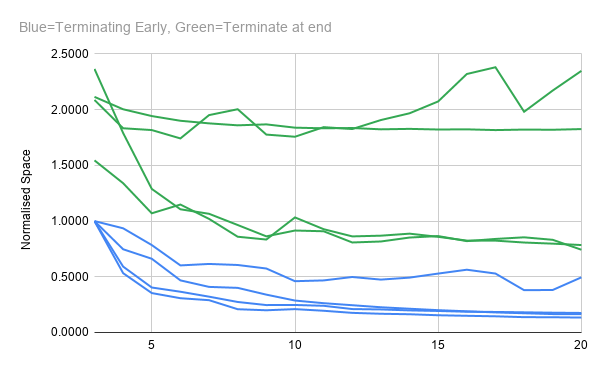
\includegraphics[width=\textwidth]{img/terminationSpace.png}
	\caption{Normalised mean space used for different termination strategies}
	%"Insertion-Only Tests"
\end{figure}
\begin{figure}
	\label{Figure 2}
  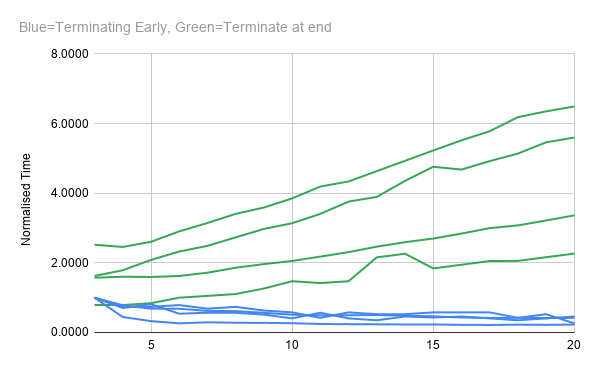
\includegraphics[width=\textwidth]{img/terminationTime.png}
	\caption{Normalised mean time taken for different termination strategies}
	%"Insertion-Only Tests"
\end{figure}
\begin{figure}
	\label{Figure 3}
  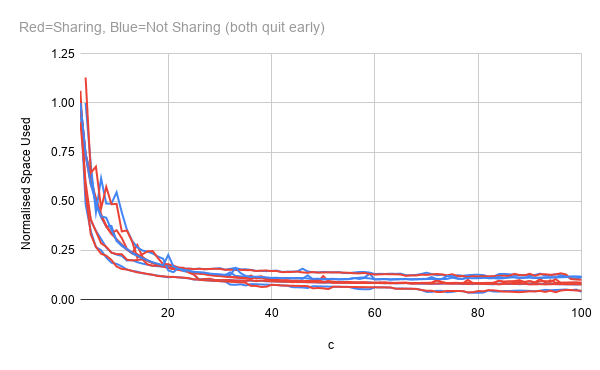
\includegraphics[width=\textwidth]{img/edgeSpace.png}
	\caption{Normalised mean space used for different edge storage strategies}
	%"Insertion-Only Tests"
\end{figure}
\begin{figure}
	\label{Figure 4}
  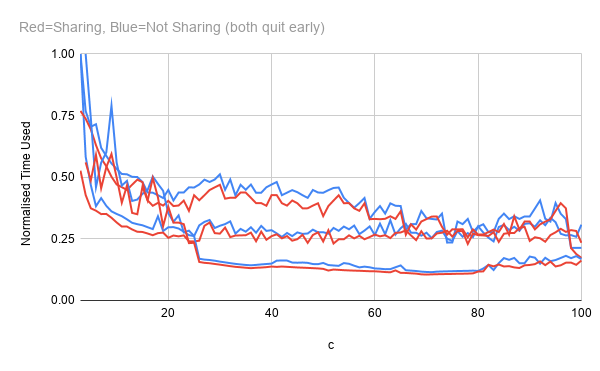
\includegraphics[width=\textwidth]{img/edgeTime.png}
	\caption{Normalised mean time taken for different edge storage strategies}
	%"Insertion-Only Tests"
\end{figure}
\begin{figure}
	\label{Figure 5}
  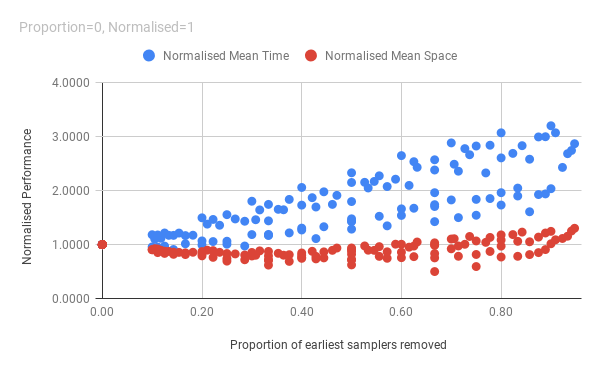
\includegraphics[width=\textwidth]{img/removedEarlySamplers.png}
	\caption{Normalised mean time-taken \& space-used when removing different proportions of the early samplers on graph \texttt{gplus}}
	%"num sampler tests"/results_removed_early_samplers_gplus
\end{figure}
\begin{figure}
	\label{Figure 6}
  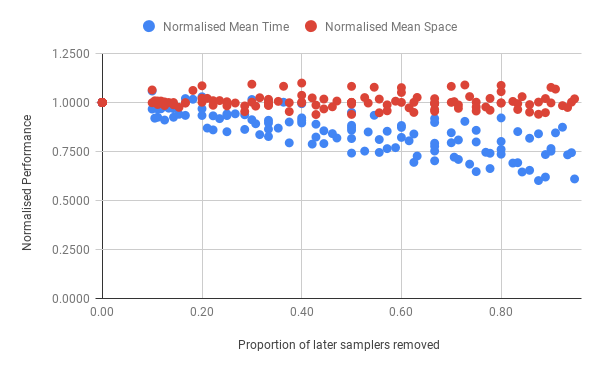
\includegraphics[width=\textwidth]{img/removedLaterSamplers.png}
	\caption{Normalised mean time-taken \& space-used when removing different proportions of the late samplers on graph \texttt{gplus}}
\end{figure}
\begin{figure}
	\label{Figure 7}
  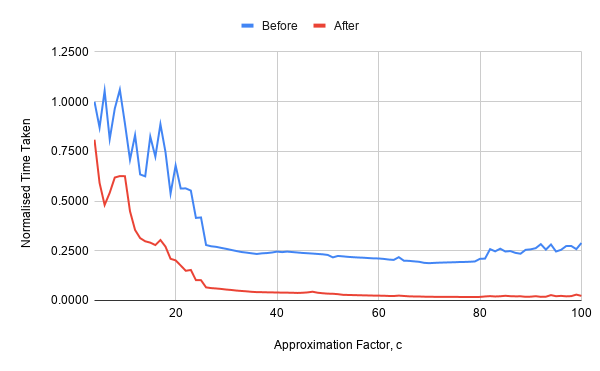
\includegraphics[width=\textwidth]{img/reducedSamplersGPlusTime.png}
	\caption{Time-taken before \& after removing late samplers from \texttt{gplus\_large}}
	%"num sampler tests"/"Compare Improvement"
\end{figure}
\begin{figure}
	\label{Figure 8}
  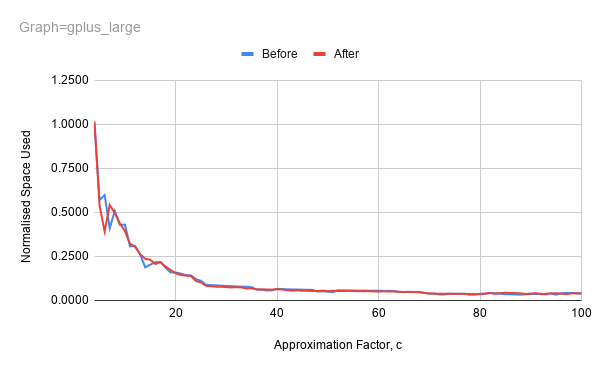
\includegraphics[width=\textwidth]{img/reducedSamplersGPlusSpace.png}
	\caption{Space-used before \& after removing late samplers from \texttt{gplus\_large}}
	%"num sampler tests"/"Compare Improvement"
\end{figure}
\begin{figure}
	\label{Figure 9}
  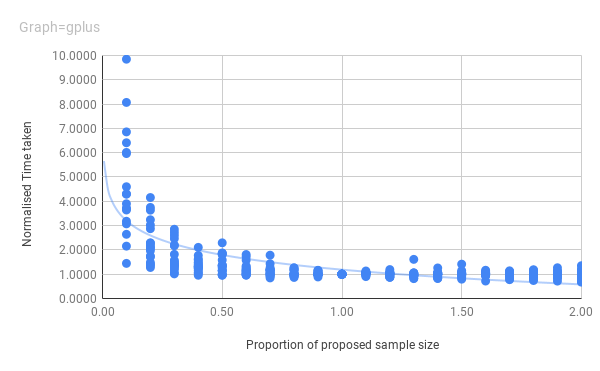
\includegraphics[width=\textwidth]{img/variedSampleSizeTime.png}
	\caption{Time-taken when varying the reservoir sample size.}
	%"sample size tests"/results_proportional_sample_size_reduction_gplus
\end{figure}
\begin{figure}
	\label{Figure 10}
	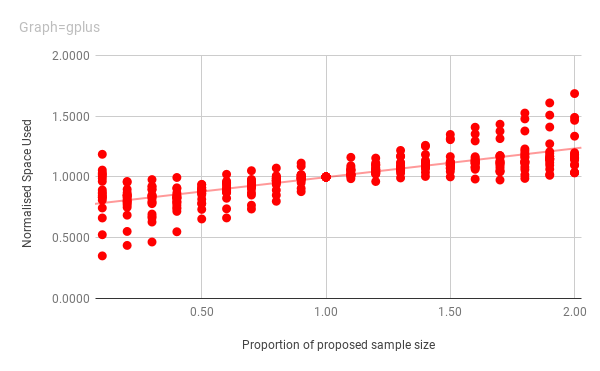
\includegraphics[width=\textwidth]{img/variedSampleSizeSpace.png}
	\caption{Space-used when varying the reservoir sample size.}
	%"sample size tests"/results_proportional_sample_size_reduction_gplus
\end{figure}
\begin{figure}
	\label{Figure 11}
	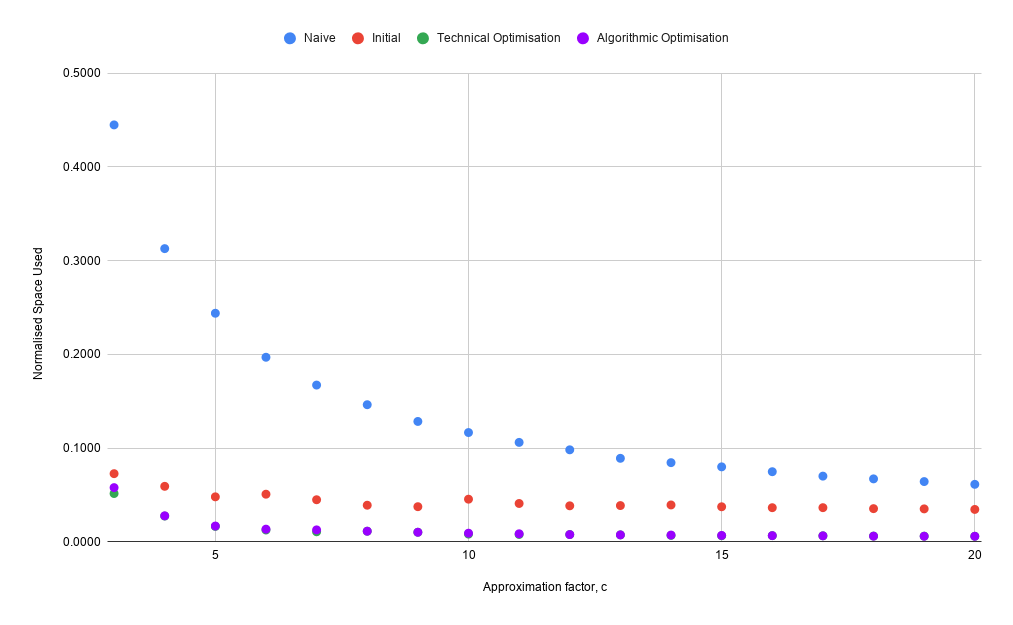
\includegraphics[width=\textwidth]{img/insertionOnlyGplusSpace.png}
	\caption{Space-used by different implementations of the algorithm for insertion-only streams when tested on \texttt{gplus}, normalised by stream size 51,839 KB}
	%"Final Evaluation - insertion-only"/Master
\end{figure}
\begin{figure}
	\label{Figure 12}
	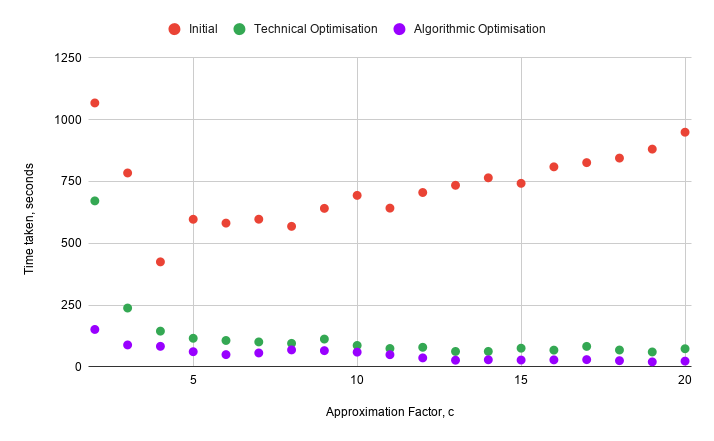
\includegraphics[width=.5\textwidth]{img/insertionOnlyGplusLargeTime1.png}
	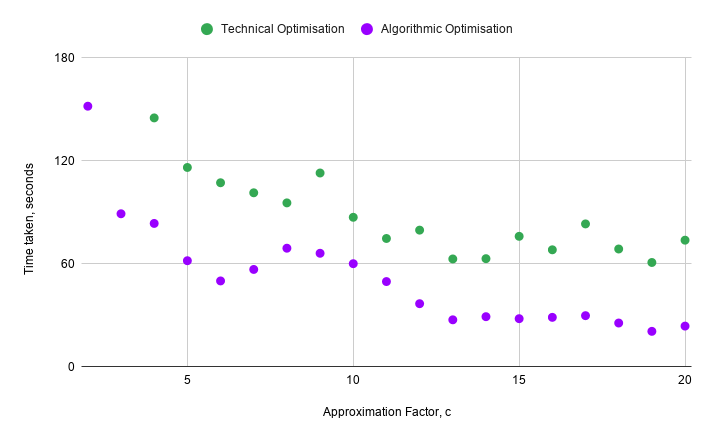
\includegraphics[width=.5\textwidth]{img/insertionOnlyGplusLargeTime2.png}
	\caption{Time-taken by different implementations of the algorithm for insertion-only streams when tested on \texttt{gplus\_large}}
	%"Final Evaluation - insertion-only"/Master
\end{figure}

\begin{thebibliography}{9}
	\addcontentsline{toc}{chapter}{Bibliography}
	\bibitem{orig} Christian Konrad \textit{Streaming Frequent Items with Timestamps and Detecting Large Neighborhoods in Graph Streams.} November 2019
	\bibitem{targetedAds} Howard Beales \textit{The Value of Behavioral Targeting}.
	\bibitem{users16} https://www.statista.com/statistics/553538/predicted-number-of-facebook-users-in-the-united-kingdom-uk/
	\bibitem{friends16} https://www.telegraph.co.uk/news/science/science-news/12108412/Facebook-users-have-155-friends-but-would-trust-just-four-in-a-crisis.html
	\bibitem{SNAP}http://snap.stanford.edu/data/
\end{thebibliography}

\end{document}
